\documentclass{beamer}

\usetheme{Madrid}
\usepackage{tikz}
\usetikzlibrary{arrows.meta, positioning}

\usepackage{minted} % For syntax-highlighted code

\title{Example Topic: Graph Traversal}
\author{Your Name}
\institute{Discrete Mathematics II, 2025S}
\date{\today}

\begin{document}

% Title slide
\begin{frame}
  \titlepage
\end{frame}

% Slide with TikZ graph
\begin{frame}{Breadth-First Search (BFS)}
Breadth-First Search is a fundamental algorithm for exploring graphs.

\begin{itemize}
  \item Explores all neighbors before going deeper
  \item Uses a queue
  \item Time complexity: \(O(V + E)\)
\end{itemize}

\vspace{0.5cm}
\begin{center}
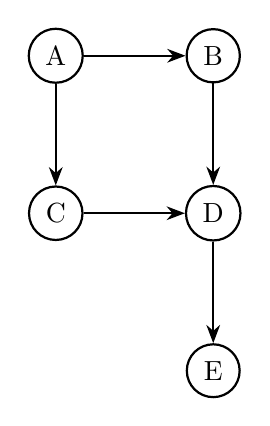
\begin{tikzpicture}[->, >=Stealth, node distance=2cm, thick]
  \node[circle, draw] (A) {A};
  \node[circle, draw, right of=A] (B) {B};
  \node[circle, draw, below of=A] (C) {C};
  \node[circle, draw, right of=C] (D) {D};
  \node[circle, draw, below of=D] (E) {E};

  \draw (A) -- (B);
  \draw (A) -- (C);
  \draw (B) -- (D);
  \draw (C) -- (D);
  \draw (D) -- (E);
\end{tikzpicture}
\end{center}
\end{frame}

% Slide with code using minted
\begin{frame}[fragile]{Python Code: BFS Example}
\begin{minted}[fontsize=\scriptsize, bgcolor=gray!5, linenos]{python}
from collections import deque

graph = {
    'A': ['B', 'C'],
    'B': ['D'],
    'C': ['D'],
    'D': ['E'],
    'E': []
}

def bfs(start):
    visited = set()
    queue = deque([start])
    while queue:
        node = queue.popleft()
        if node not in visited:
            print(node, end=' ')
            visited.add(node)
            queue.extend(graph[node])

bfs('A')
\end{minted}
\end{frame}

\end{document}
